\chapter{Warm core rings release predators from thermal constraints when foraging in the ocean Twilight zone}
\label{chap:5}
\raggedbottom


{\let\thefootnote\relax\footnotetext{This chapter is constructed as a short format manuscript awaiting submission as Braun, C.D., Gaube P., Sinclair-Taylor T., Skomal, G.B., and Thorrold S.R. Warm core rings release predators from thermal constraints when foraging in the ocean Twilight zone.}}
%\end{singlespace}
{\let\thefootnote\relax\footnotetext{C.D.B. and S.R.T. designed the study. C.D.B, T.S.T. and G.B.S. conducted the tagging; C.D.B. performed the analysis with contributions from P.G. and S.R.T. C.D.B. wrote the paper with contributions and final approval from all authors.}}

\begin{comment}

Warm core rings release predators from thermal constraints when foraging in the ocean Twilight zone

\textbf{Camrin D. Braun$^{1,2}$, Peter Gaube$^3$, Tane Sinclair-Taylor$^4$, Gregory B. Skomal $^5$ \& Simon R. Thorrold$^2$}

\footnotesize
\begin{enumerate}
\item Massachusetts Institute of Technology-Woods Hole Oceanographic
  Institution Joint Program in Oceanography/Applied Ocean Science and
  Engineering, Cambridge, MA 02139, USA
\item Biology Department, Woods Hole Oceanographic Institution, Woods Hole,
  MA 02543, USA
\item Air-Sea Interaction and Remote Sensing Department, Applied Physics
  Laboratory - University of Washington, Seattle, WA, 98105, USA
\item Red Sea Research Center, Division of Biological and Environmental Sciences and Engineering, King Abdullah University of Science and Technology, Thuwal 23955-6900, Saudi Arabia
\item Massachusetts Division of Marine Fisheries, 836 South Rodney French
  Blvd., New Bedford, MA 02744, USA
\end{enumerate}
\end{comment}


\clearpage

\section{Abstract} 

%% ABSTRACT

%fully referenced paragraph, ideally of about 200 words, but certainly no more than 300 words, aimed at readers in other disciplines. This paragraph starts with a 2-3 sentence basic introduction to the field; followed by a one-sentence statement of the main conclusions starting 'Here we show' or equivalent phrase; and finally, 2-3 sentences putting the main findings into general context so it is clear how the results described in the paper have moved the field forwards.

Mesoscale eddies comprise the "internal weather" of the ocean and can generate first order perturbations of open ocean ecosystems \citep{Mahadevan2014, McGillicuddy2007}. The Gulf Stream generates some of the most energetic eddies and meanders found anywhere in the global ocean.  Counterclockwise-rotating cyclonic eddies trap cold, nutrient-replete water from north of the Gulf Stream during formation and clockwise-rotating anticyclonic eddies characterized by anomalously warm water that is low in chlorophyll and nutrients due to its source in the northern Sargasso Sea \citep{Gaube2017DSR}. Using new observations from pelagic predators and a constellation of earth-observing satellites, our results challenge the existing paradigm that anticyclonic eddies are ocean "deserts" characterized by anomalously warm water and generally low phytoplankton biomass \citep{Gaube2017DSR, Williams1998}. Here, we show that blue sharks (\textit{Prionace glauca}), a model epipelagic predator, actively seek out the interiors of anticyclonic Gulf Stream eddies where they most often exhibit behaviors indicative of foraging. Using > 2,000 tracking days and nearly 500,000 high-resolution time series measurements collected by 15 instrumented blue sharks, we show that these "evolutionarily-informed oceanographers" regularly dive deep into the mesopelagic (> 200 m) in anticyclones where anomalously warm temperatures alleviate a physiological constraint that otherwise isolates mesopelagic fish biomass from many epipelagic predators. Anticyclonic eddies thus provide a conduit by which surface-oriented predators access the most abundant fish community on the planet \citep{Irigoien2014}. The results presented here provide valuable new insight into open ocean habitat use by large pelagic predators that should be incorporated into dynamic ocean management approaches. Furthermore, our results shed new light onto the ecosystem value of mesopelagic prey, suggesting additional considerations are necessary before planned biomass extraction from the Ocean's twilight zone as these activities could interrupt a key link between planktonic production and top predators \citep{Smith2011}.

%% MAIN TEXT
% rest of the text is typically about 1,500 words long, including body text and methods summary
% typically 3-4 figures and tables total
\clearpage
\section{Main Text} 

The pelagic ocean represents the largest habitat on Earth \citep[99\% of the biosphere][]{Game2009} and yields >80\% of the fish consumed by humans \citep{Game2009,Pauly2002}. Mesoscale eddies are ubiquitous, energetic features that structure open ocean ecosystems \citep{McGillicuddy2016} on time scales of weeks to months and spatial scales $\mathcal{O}$(10s - 100s km). These features are known to control biogeochemical fluxes and transport entire pelagic communities \citep{Chelton2011}. While eddies are known to affect biological communities from plankton \citep{McGillicuddy2007, benitez2007mesoscale} to predators \citep{Bailleul2010,Gaube2018}, studies of the coupling of biology and ocean physics at the oceanic mesoscale remain inconclusive with respect to the role of anticyclones in maintaining preferential foraging conditions for upper trophic levels. Fish communities, in particular, are difficult to quantitatively link to mesoscale oceanographic features due to constraints imposed by traditional light-level geolocation \citep[][Chapter \ref{chap:2}]{Braun2018a}. Yet, if fishes are able to sense favorable conditions associated with mesoscale eddies as has been shown for turtles \citep{Gaube2017, Kobayashi2011}, seabirds \citep{TewKai2009}, mammals \citep{Bailleul2010}, and indeed large white sharks \citep{Gaube2018}, eddies may have profound impacts on many commercially- and ecologically-important fish species.

Recent advances in satellite oceanography have facilitated the automatic identification and tracking of mesoscale eddies. Cyclonic eddies (CEs) in this region (including those generated by the Gulf Stream known as cold-core rings) typically trap cold, productive water from the New England shelf during formation \citep{Pingree1979, RingGroup1981} while anticyclones (ACEs, or warm-core rings) transport anomalously warm, low productivity Sargasso Sea water north of the Gulf Stream \citep{Joyce1985, Franks1986}. Due to these characteristics, ACEs are often characterized as warm, ocean "deserts" void of significant productivity \citep{Williams1998}, particularly in the Gulf Stream \citep{Gaube2014}. Recent work on predators in this region suggests that white sharks \citep{Gaube2018} and swordfish (Chapter \ref{chap:4}) may preferentially occupy anticyclones, but inference in these studies was limited by sample size and fisheries-dependence, respectively. Here we report high-resolution, three-dimensional movements of 15 blue sharks in the Gulf Stream eddy field. The results document preferred occupation of the cores of anticyclonic eddies, particularly while sharks exhibited horizontal movements indicative of foraging, that are counter to the paradigm of low biomass in open ocean anticyclones. Diving behavior in these features demonstrated the thermal constraints operating on an ectothermic, seemingly epipelagic predator and highlight unrecognized connections between epipelagic predators and mesopelagic prey that are modulated by ocean dynamics.

%-------------------------
\begin{figure}[htbp]
\centering
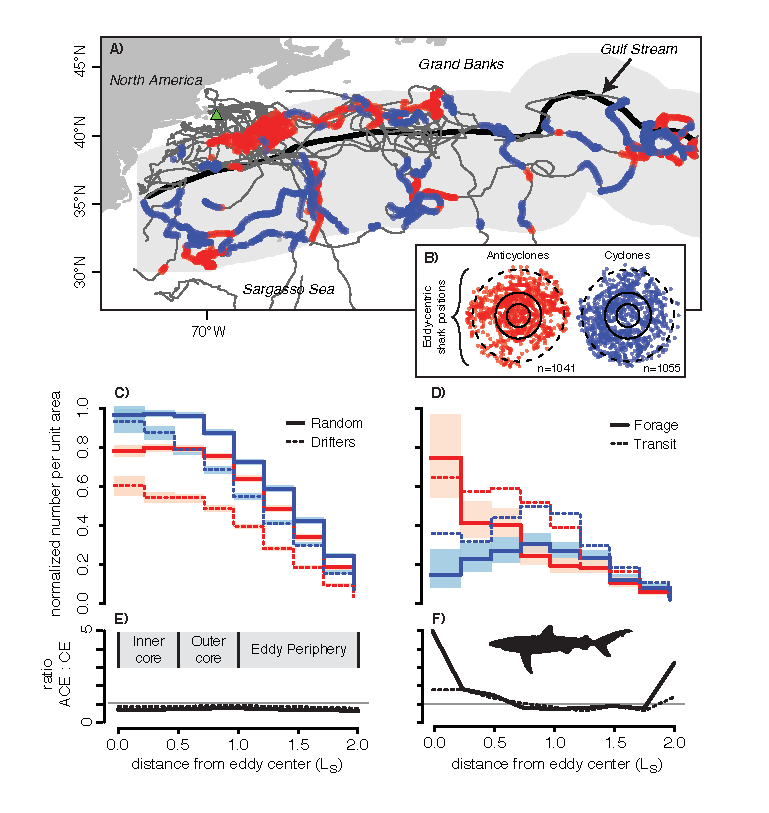
\includegraphics{images/C5_Fig1.pdf}
\caption[Use of Gulf Stream eddies by satellite-tagged blue sharks]{Blue sharks tagged in New England frequented the Gulf Stream eddy field (A) and occupied anticyclones (red throughout) and cyclones (blue throughout) at approximately the same frequency (B). Eddy-centric histograms indicated random walk simulations (solid, C) and passive drifters (dashed, C) exhibited higher cyclone use after controlling for eddy area. Sharks (D) used eddy peripheries ($>L_s$) approximately equally between eddies of either polarity, but more positions classified as "transiting" (dashed, D) were collocated around the eddy length scale ($L_s$) compared to "foraging" locations (solid, D). Sharks showed a marked preference for the cores of anticyclones relative to cyclones, particularly while foraging (D). The ratio of anticyclone (ACE) to cyclone (CE) positions across different regions of the eddies are shown for random walk simulations (E), drifters (E) and foraging (solid) and transiting (dashed) modes in the shark data (F). Note confidence intervals have been removed from the transit mode in panel D to aid visualization.}
\label{fig:c5f1}
\end{figure}
%-------------------------

We instrumented 15 blue sharks each with 2 types of satellite tags: a satellite-linked position transmitter (SPOT tag) mounted on the dorsal fin and a pop-up satellite archival transmitting (PSAT) tag that recorded high-resolution depth and temperature time series. Two additional sharks were tagged with SPOT tags only. All 17 SPOT tags reported a total of 8,279 positions over 2,117 tracking days (mean 4 positions $\cdot$ day $^{-1}$; deployment duration range 54-288 days). A hierarchical state-space movement model was used to delineate behaviors in the movement data indicative of "foraging" (area-restricted search) and "transiting" based on correlation and turn angles \citep{Jonsen2016}. Movements were combined with $\sim$482,000 depth and temperature time series data points at 2.5 minute resolution from 12 PSAT tags at liberty for an average 129 days (range 16-180) to reconstruct blue shark movements in 3D. On average, overall movements covered 5,454 km (range 2,280-14,485 km) in up to 288 days at liberty and were predominantly oriented east-west at temperate latitudes (Fig. \ref{fig:c5f1}A). PSAT-tagged sharks made extensive vertical movements offshore where they regularly dove to at least 400 m (maximum depth 1,696 m), almost exclusively during daylight hours (Fig. \ref{fig:c5f2}). Sharks occupied a 26$^\circ$C temperature range (mean 18.5$^\circ$C, range 4.0-29.6$^\circ$C) but remained above the 12$^\circ$C isotherm while diving (97\% of temperature data > 12$^\circ$C; Figs. \ref{fig:c5f2}, \ref{fig:c5f3}), suggesting thermal constraints prevented use of colder water \citep{Carey1990}.

Blue shark movements and depth-temperature time series data were collocated to mesoscale eddies in the Gulf Stream tracked in maps of sea level anomaly. Area-normalized histograms of shark positions as a function of distance from eddy centers revealed that blue sharks were significantly more likely to be associated with the inner-cores ($r \leq L_s / 2$) of ACEs than CEs (Fig. \ref{fig:c5f1}). The preference for ACEs was further strengthened when considering only the foraging behavior mode (Fig. \ref{fig:c5f1}D). Depth-temperature time series data indicated a total of 15,189 depth measurements were made within eddies representing 452 and 181 cumulative hours within anticyclonic and cyclonic eddy cores ($r \leq L_s$), respectively. Distribution of time-at-depth in eddies was indicative of blue sharks foraging on diel vertically-migrating, mesopelagic prey during dives as sharks spent 15\% of time in ACEs below 300 m compared to 1.5\% in Gulf Stream CEs during day and < 1\% in eddies of either polarity during night (Fig. \ref{fig:c5f2}E,F). While diving, tagged individuals encountered strong positive (warm) temperature anomalies at depth in ACEs (Figs. \ref{fig:c5f2}, \ref{fig:a5f1}, \ref{fig:a5f2}), including as high as +10$^\circ$C from 250-350 m (Fig. \ref{fig:a5f1}). Blue sharks experienced significant negative temperature anomalies at depth in some cyclones as predicted by vertical eddy composites (Figs. \ref{fig:c5f2}, \ref{fig:a5f1}, \ref{fig:a5f2}); however, the majority of diving in CEs occurred in water warmer than that suggested by eddy vertical composites (Fig. \ref{fig:c5f2}B) or known upward vertical displacement of isotherms typical of Gulf Stream CEs \citep[cold-core rings;][]{Gaube2014, Gaube2018}. Tracking the warm eddies back to their formation indicated these warm CEs were of Sargasso Sea origin and had moved into the southern portion of the Gulf Stream study area. Further analysis confirmed sharks occupied very few traditional cold-core rings generated by the Gulf Stream (Fig. \ref{fig:c5f3}E,F) in favor of warm Sargasso-derived CEs instead.

\clearpage

%Instead, diving in CEs was within $\pm$ 2$^\circ$C of climatological mean temperatures at depth (Fig. \ref{fig:vert}) and the vertical structure of these cyclones were nearly indistinguishable from warm ambient water south of the GS (Fig. \ref{fig:ex}). \textbf{**Pete, insert here about mode-2 CEs**. }
%-------------------------
\begin{landscape}
\begin{figure}[htbp]
\centering
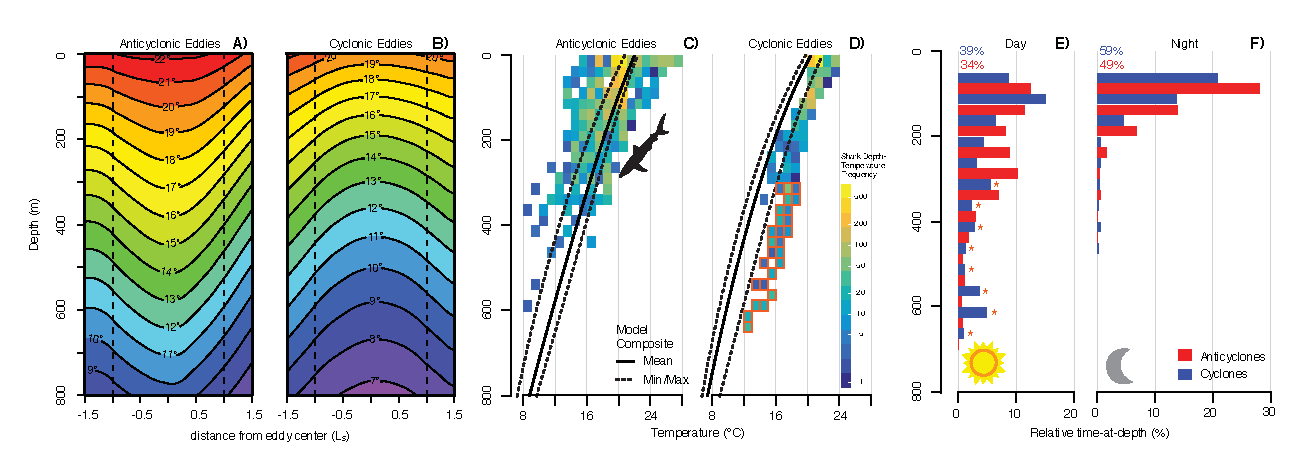
\includegraphics[width=9in]{images/C5_Fig2.pdf}
\caption[Eddy vertical structure and blue shark diving]{Eddy vertical structure and blue shark diving. Modeled depth-temperature profile composites for 27 anticyclonic (A) and 28 cyclonic (B) eddies occupied by blue sharks. Histogram of blue shark depth-temperature data while diving in cores ($r < L_s$) of anticyclones (C; n=7,271) and cyclones (D; n=2,521) compared to model composite depth-temperature profiles. Summary of blue shark time-at-depth during day (E) and night (F) occupation of anticylonic (red) and cyclonic (blue) eddies. The 0-50m depth bin has been removed to aid visualization. The highlighted depth-temperature cells (orange outline, D) and time-at-depth bins (orange asterisks, E) correspond to diving in cyclones of Sargasso Sea origin.}
\label{fig:c5f2}
\end{figure}
\end{landscape}
\clearpage
%-------------------------

The observed differences in temperature at depth among ACEs, Gulf Stream CEs and Sargasso-derived CEs regulated the blue shark diving in these eddies (Fig. \ref{fig:c5f3}A-C), primarily by modulating the depth of the 12$^\circ$C isotherm (Fig. \ref{fig:c5f3}E,F). We developed a metric ($D'$; Eq. \ref{eq:a5dprime}) to quantify the relationship between shark maximum dive depth relative to the climatological mean depth of the 12$^\circ$C isotherm in which $D'$>0 is indicative of anomalously deep diving relative to the climatological mean. This analysis found diving in ACEs was primarily characterized by $D'$>0 while CEs more often exhibited $D'$<0 (Fig. \ref{fig:c5f3}E), suggesting eddy modulation of water column structure controlled shark behavior in these features. This was confirmed by comparing climatological mean depth of the 12$^\circ$C isotherm to modeled \is depth in eddies (Fig. \ref{fig:c5f3}F).

Our results suggest that blue sharks synthesize an evolutionary "knowledge" of high biomass in the mesopelagic with the constraints of their thermal physiology by using warm, anticyclonic eddies as conduits to the deep ocean. This contrasts with the ocean "desert" paradigm of anticyclonic eddies but corroborates recent observations that, in contrast to their low chlorophyll surface signature, ACEs can contain among the highest deep scattering layer densities in the world oceans \citep{Fennell2015}. In addition, other recent work has shown that some specific types of ACEs contain enhanced primary productivity in their cores \citep{Dufois2016}. While we are unable to attribute specific behaviors to \textit{P. glauca} during dives, previous studies tracking blue sharks in the Gulf Stream reported a high frequency of octopods, a diel vertical migrator that occurs principally below 250 m, in blue shark stomachs \citep{Carey1990}. In addition, mesopelagic dives by blue sharks were nearly always during daytime when the bulk of the mesopelagic community is at depth \citep{Bianchi2013}, and shark dive profiles were characterized by rapid descents with slower ascents, a pattern interpreted as prey searching behavior in sharks and tunas \citep{Carey1990, Brunnschweiler2009}. Taken together, deep dives suggest blue sharks are foraging for cephalopods and mesopelagic fishes, some of the blue sharks primary prey items \citep{Nakano2008}, that are known to concentrate at depth in the Gulf Stream \citep{Fedulov1986} and have been collected in high densities in ACEs \citep{Fennell2015, godo2012mesoscale}. However, additional research will be needed to confirm this hypothesis.

%-------------------------
\begin{figure}[htbp]
\centering
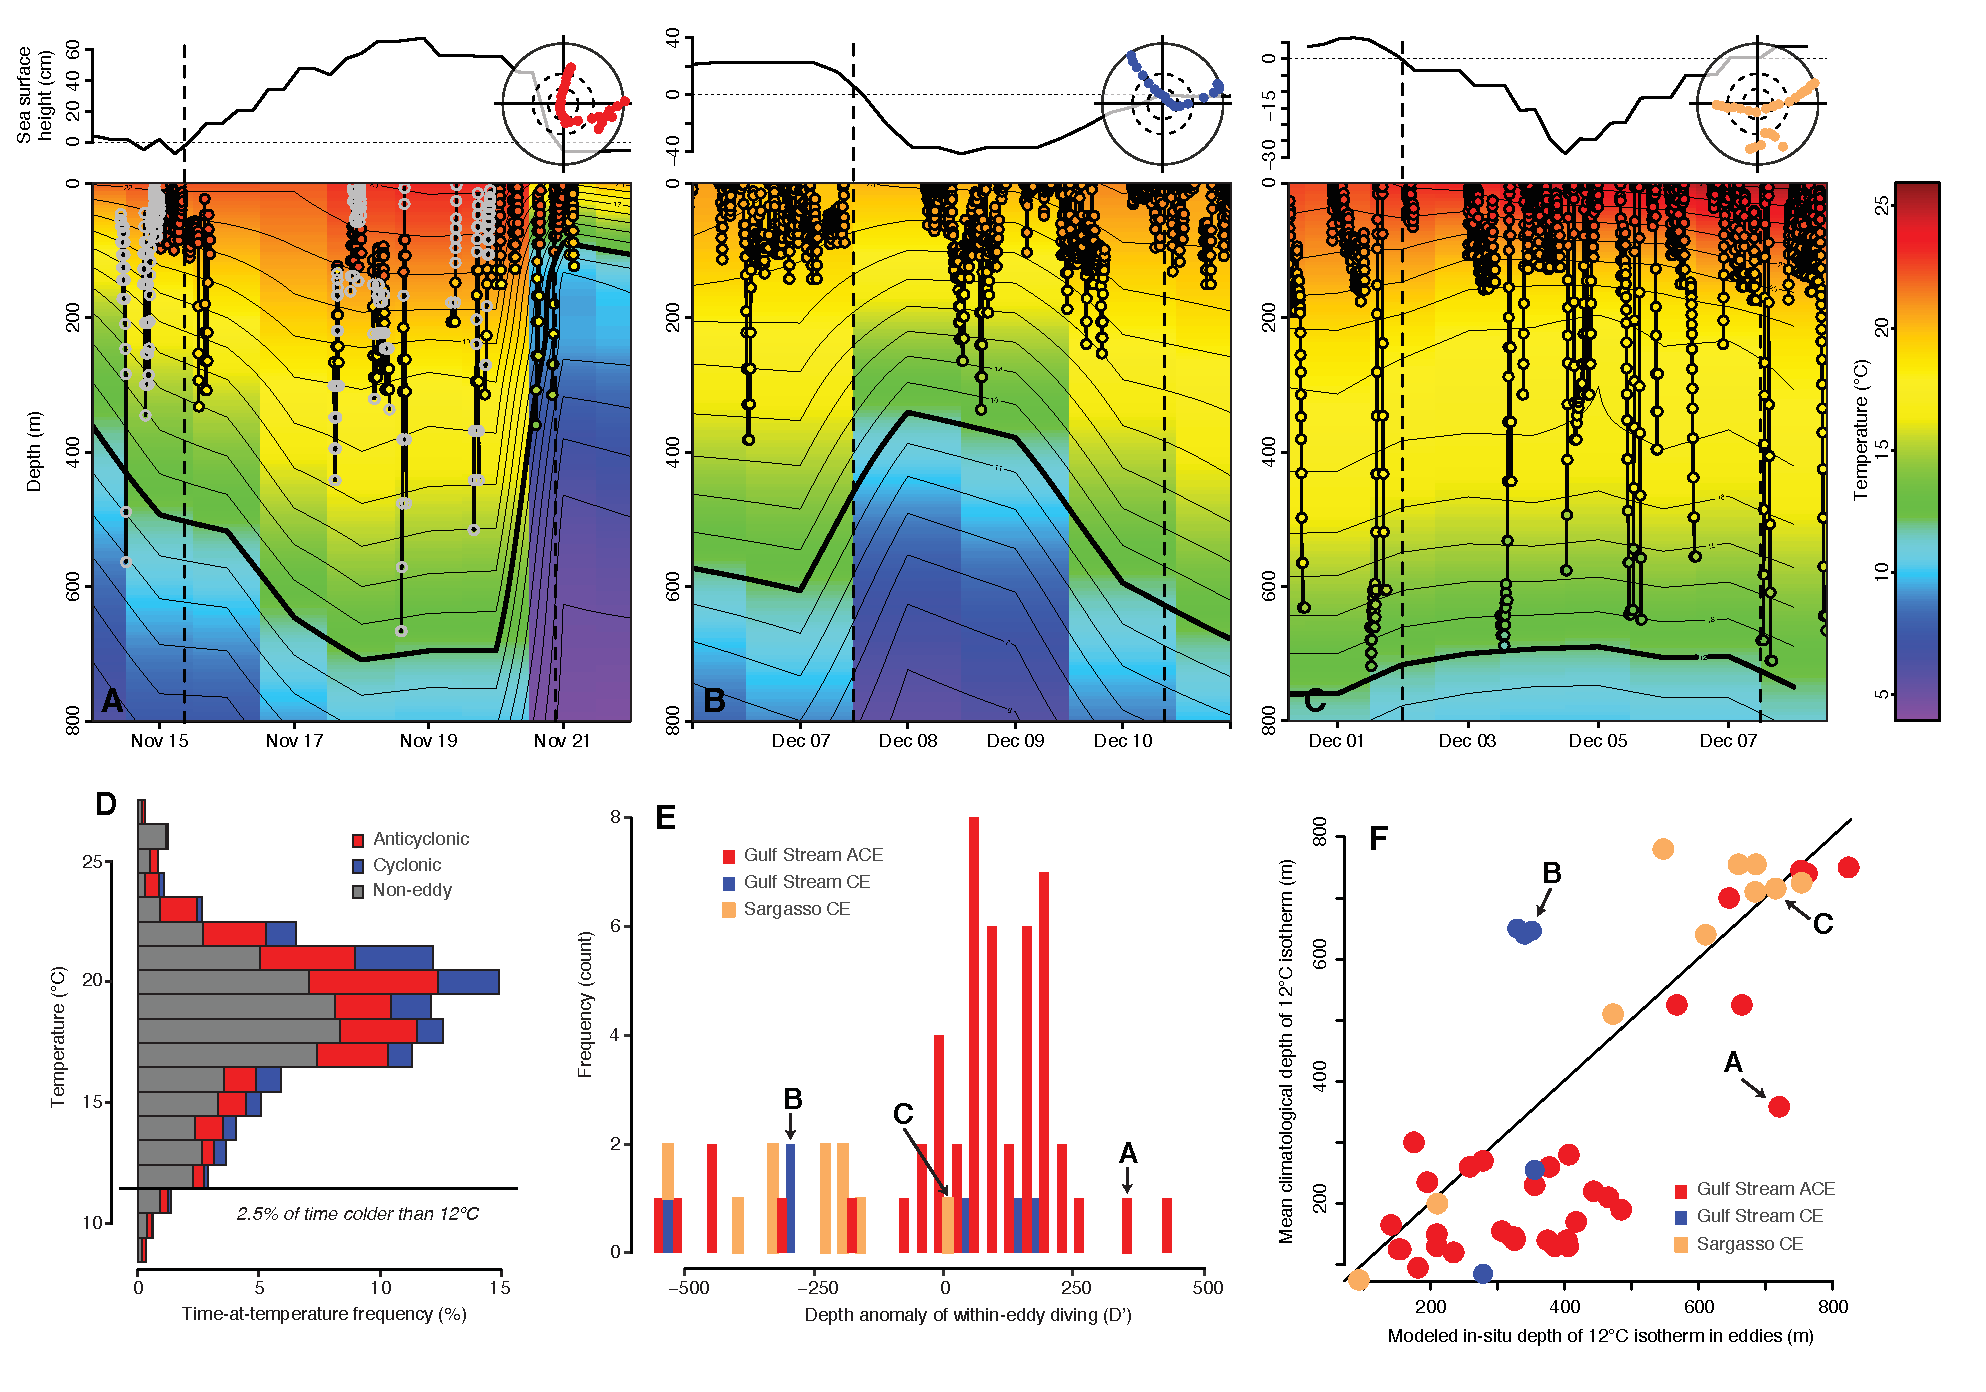
\includegraphics[width=\textwidth]{images/C5_Fig3.pdf}
\caption[Example diving by blue sharks in Gulf Stream eddies and a Sargasso Sea cyclone]{Example diving by blue sharks in anticyclonic (A) and cyclonic (B) Gulf Stream eddies and a cyclonic eddy of Sargasso Sea origin (C). Upper line plots indicate measured sea surface height from AVISO (Eqn. \ref{eq:a5ssh}). Top right circular plots in each panel show geographic movements of the shark in eddy-centric coordinates (as in Fig. \ref{fig:c5f1}). Water column structure in the eddies (color map, top panels) is modeled depth-temperature data from HYCOM. Colored points connected by solid vertical lines represent shark diving behavior (grey circles indicate no temperature data was acquired/transmitted by the tag for a given depth point in the time series). Dashed vertical lines indicate entry and exit of eddies based on SSH. Thin, labeled horizontal lines indicate isotherms at 1$^\circ$C intervals. Frequency histogram of the time-at-temperature distribution for all shark dive data in the Gulf Stream (D) and for the depth anomaly of within-eddy diving (E; see Eq. \ref{eq:a5dprime}). Positive $D'$ indicates sharks dove below the climatological 12$^\circ$C isotherm, suggesting vertical downward displacement of isotherms by the eddy as shown by comparing climatological mean isotherm depth to \is modeled isotherm depth within eddies (F).}
\label{fig:c5f3}
\end{figure}
%-------------------------

While the mesopelagic contains the highest fish biomass on earth \citep{Irigoien2014}, the deep ocean presents significant physiological challenges for epipelagic predators. ACEs may provide a unique conduit from the surface to deep ocean due to anomalously warm temperatures at depth where high acoustic scattering (a proxy for prey availability or biomass) at depth has been shown to have a strong positive correlation with temperature \citep{Fennell2015}. While Gulf Stream cyclones can contain significant productivity \citep{Gaube2017DSR}, our data suggest the thermal constraints to diving in these features disconnect the epi- and mesopelagic fish communities. Indeed, recent work has suggested endothermic white sharks are likely able to forage deep in Gulf Stream cyclones but that dive times are shorter than in ACEs \citep{Gaube2018}. Previous studies have suggested the thermoregulatory implications of deep diving for several epipelagic predators, including elasmobranchs \citep{Thorrold2014}, marine mammals \citep{Tyack2006} and commercially-important fishes \citep{Carey1982}. Work on blue sharks suggests thermal hysteresis facilitates maintenance of body temperatures significantly above ambient in the mesopelagic followed by abrupt termination of deep dives when muscle cools to <15$^\circ$C \citep{Carey1990}. We observed similar oscillatory diving into the mesopelagic during daytime in both types of Gulf Stream eddies that was seemingly constrained by temperature at depth (Fig. \ref{fig:c5f3}), consistent with the behavioral thermoregulation observed by \cite{Carey1990}. Sharks spent more time deeper in ACEs (Fig. \ref{fig:c5f2}) than CEs, regularly as deep as 300-350 m, where backscatter is reportedly high \citep{Fennell2015} and temperatures were consistently >12$^\circ$C. Thus, it seems the potentially enhanced foraging opportunities combined with relaxing of thermal constraints in ACEs may interact to drive blue shark preference for these features.

Our results highlight the potential role of oceanography in modulating the connectivity between epipelagic predator communities and the twilight zone. This region has proven particularly difficult to study but likely supports a number of commercially-important fishes (such as sharks, swordfish and tunas) and may provide significant support for open ocean foodwebs. We show that dynamic mesoscale eddies modulate this connection, yet current management approaches largely ignore the highly dynamic ocean in favor of traditional, static management approaches \citep{Maxwell2015}. Finally, we provide additional evidence of the value of mesopelagic communities to pelagic predators, suggesting extraction of deep ocean resources may interrupt this key resource.

%-------------------
\section*{METHODS SUMMARY}

Detailed methods and supporting figures and tables can be found in Appendix \ref{sec:app5}.

\subsection*{Satellite tagging and track analysis}
Blue sharks were tagged with electronic tags that provided both accurate (< 10 km error) satellite-based positions and a time series of depth and temperature every 2.5 minutes. Locations were filtered to remove spurious positions and data gaps > 4 days. Filtered tracks were fit in a hierarchical fashion with a two-state switching state-space model to standardize the location time series and infer behavior state \citep{Jonsen2016}. Resulting positions were used to collocate depth and temperature data for reconstruction of 3D movements.

\subsection*{Eddies}
Eddies were identified and tracked in daily maps of surface altimetry. A custom meander filter was used to remove Gulf Stream meanders before shark movement data was collocated to the nearest identified eddy in the atlas. Eddy subregions were defined according to the radial distance from the eddy center \citep{Gaube2017}. Null eddy use was quantified by two independent methods: shark movements simulated by random walks and 5 years of surface drifter data. Eddy vertical composites were constructed for shark-occupied eddies using HYCOM modeled depth-temperature profiles and anomalies used climatological mean temperature from the World Ocean Atlas.

